% Copyright (C) 2005-2015 Airbus - EDF - IMACS - Phimeca
% Permission is granted to copy, distribute and/or modify this document
% under the terms of the GNU Free Documentation License, Version 1.2
% or any later version published by the Free Software Foundation;
% with no Invariant Sections, no Front-Cover Texts, and no Back-Cover
% Texts.  A copy of the license is included in the section entitled "GNU
% Free Documentation License".
\renewcommand{\filename}{docUC_StocProc_DensitySpectralModel_Estimation.tex}
\renewcommand{\filetitle}{UC : Estimation of a spectral density function}

% \HeaderNNIILevel
% \HeaderIILevel
\HeaderIIILevel

\index{Stochastic Process!Spectral Model}

Let $X: \Omega \times \cD \rightarrow \Rset^d$  be a multivariate  stationary normal process of dimension $d$. We only treat here the case where the domain is of dimension 1: $\cD \in \Rset$ ($n=1$). \\
If the process is continuous, then $\cD=\Rset$. In the discrete case, $\cD$  is a lattice. \\


$X$ is supposed to be a second order process with zero mean and we suppose that its spectral density function $S : \Rset \rightarrow \mathcal{H}^+(d)$ defined in (\ref{specdensFunc}) exists. $\mathcal{H}^+(d) \in \mathcal{M}_d(\Cset)$ is the set of $d$-dimensional positive definite hermitian matrices.\\


This objective of this use case is to estimate the spectral density function $S$ from data, which can be a sample of time series or one time series.\\
Depending on the available data, we proceed differently :
\begin{itemize}
\item if the data correspond to  several independent  realizations of the  process (stored in a \textit{ProcessSample} object), a \emph{statistical estimate} is performed using statistical average of a realization-based estimator;
\item if the data correspond to one realization of the  process  at different time stamps (stored in a  \textit{TimeSeries} object), the process being observed during a long period of time, an \emph{ergodic estimate} is performed using a time average of an ergodic-based estimator.
\end{itemize}

The estimation of the spectral density function from data may use some parametric or non parametric methods. \\
The \textit{Welch} method is a \emph{non parametric} estimation technique, known to be performant. We detail it in the case where the available data on the process is a time series which values are $(\vect{x}_0, \dots,\vect{x}_{N-1})$ associated to the time grid $(t_0, \dots, t_{N-1})$ which is a discretization of the domain $[0,T]$.\\
We assume that the process has a spectral density $S$ defined on $| f | \leq \frac{T}{2}$.\\

The method is based on the segmentation of the time series into $K$ segments of length $L$, possibly overlapping (size of overlap $R$).\\
Let $\vect{X}_{1}(j), \ j = 0, 1,...,L-1$ be the first such segment. Then :
\begin{equation*}
  \vect{X}_{1}(j) = \vect{X}(j) , \ j = 0, 1,...,L-1
\end{equation*}
Applying the same decomposition,
\begin{equation*}
  \vect{X}_{2}(j) = \vect{X}(j + (L - R)) , \ j = 0, 1,...,L-1
\end{equation*}
and finally :
\begin{equation*}
  \vect{X}_{K}(j) = \vect{X}(j + (K-1)(L-R)) , \ j = 0, 1,...,L-1
\end{equation*}

The objective is to get a statistical estimator from these $K$ segments. We define the \emph{periodogram} associated with the segment $\vect{X}_k$ by:
\begin{eqnarray*}
  \vect{X}_{k}(f_p,T)&=&\Delta t\sum_{n=0}^{L-1}\vect{x}(n\Delta t)\exp\left[\frac{-j2\pi pn}{N}\right], \quad p=0,\dots, L-1\\
  \hat{G}_{\vect{x}}(f_p,T)&=&\frac{2}{T}\vect{X}_{k}(f_p,T)\,{\vect{X}_{k}(f_p,T)^*}^t,\quad p=0,\dots,L/2-1
\end{eqnarray*}
with $\Delta t=\frac{T}{N}$ and $f_p=\frac{p}{T}=\frac{p}{N}\frac{1}{\Delta t}$.\\

It has been proven that the \emph{periodogram} has bad statistical properties. Indeed, two quantities summarize the properties of an estimator:
its \emph{bias} and its \emph{variance}.
The bias is the expected error one makes on the average using only a finite number of time series of finite length, whereas the covariance is the expected fluctuations of
the estimator around its mean value. For the periodogram, we have:

\begin{itemize}
\item Bias$=\mathbb{E}[\hat{G}_{\vect{x}}(f_p, T)-G_{\vect{X}}(f_p)]=(\frac{1}{T}W_B(f_p, T)-\delta_0)*G_{\vect{X}}(f_p)$ where $W_B(f_p, T) = \left(\frac{\sin\pi fT}{\pi fT}\right)^2$ is the squared module of the Fourier transform of the function $w_B(t, T)$ (\emph{Barlett window}) defined by:
  \begin{equation}
    w_B(t, T) = \mathbf{1}_{[0,T]}(t)
  \end{equation}
  This estimator is \emph{biased} but this bias vanishes when $T\rightarrow\infty$ as $\lim_{T\rightarrow\infty} \frac{1}{T}W_B(f_p, T)=\delta_0$.
\item Covariance$=\frac{1}{T}W_B(f_p, T)*G_{\vect{X}}(f_p)\rightarrow G_{\vect{X}}(f_p)$ as $T\rightarrow\infty$,
  which means that the fluctuations of the periodogram are of the same order of magnitude as the quantity to be estimated and thus the estimator is not convergent.
\end{itemize}

The periodogram's lack of convergence may be easily fixed if we  consider the \emph{averaged periodogram} over $K$ independent time series or segments:
\begin{equation}
  \hat{G}_{\vect{x}}(f_p,T)=\frac{2}{KT}\sum_{k=0}^{K-1}\vect{X}^{(k)}(f_p,T)\vect{X}^{(k)}(f_p,T)^t
\end{equation}

The averaging process has no effect on the significant bias of the periodogram.

The use of a \emph{tapering window} $w(t, T)$ may significantly reduce it. The time series $\vect{x}(t)$ is replaced by a tapered time series $w(t, T)\vect{x}(t)$ in the
computation of $\vect{X}(f_p,T)$. One gets :
\begin{equation}
  \mathbb{E}[\hat{G}_{\vect{x}}(f_p, T)-G_{\vect{X}}(f_p)=(\frac{1}{T}W(f_p, T)-\delta_0)*G_{\vect{X}}(f_p)
\end{equation}
where $W(f_p, T)$ is the square module of the Fourier transform of $w(t, T)$ at the frequency $f_p$.
A judicious choice of tapering function such as the \emph{Hanning window} $w_H$ can dramatically reduce the bias of the estimate:
\begin{equation}\label{HamEff}
  w_H(t, T) = \sqrt{\frac{8}{3}}\left(1-\cos^2\left(\frac{\pi t}{T}\right)\right)\mathbf{1}_{[0,T]}(t)
\end{equation}

OpenTURNS builds an estimation of the spectrum on a \textit{TimeSeries} by fixing the number of segments, the \textit{overlap} size parameter and a \textit{FilteringWindows}. The available ones are :
\begin{itemize}
\item The \textit{Hamming} window
  \begin{equation}
    w(t, T) = \sqrt{\frac{1}{K}}\left(0.54-0.46\cos^2\left(\frac{2 \pi t}{T}\right)\right)\mathbf{1}_{[0,T]}(t)
  \end{equation}
  with $K$ = $\sqrt{0.54^2 + \frac{1}{2} 0.46^2}$
\item The \textit{Hanning} window described in (\ref{HamEff}) which is supposed to be the most usefull.
\end{itemize}
The result consists in a \textit{UserDefinedSpectralModel} which is simple to manipulate. \\

Furthermore, OpenTURNS build an estimation of the spectral function on a process sample by considering that $k-th$ segment is the $k-th$ time series  of the process sample .
User should pay attention that data must be centred otherwise user could center them himself. \\


\requirements{

  \begin{description}
  \item[$\bullet$] number of segments {\itshape mySegmentNumber}
  \item[type:]  integer
  \end{description}

  \begin{description}
  \item[$\bullet$] size of overlap {\itshape myOverlapSize}
  \item[type:]  integer
  \end{description}

  \begin{description}
  \item[$\bullet$] a time series {\itshape myTimeSeries}
  \item[type:]  TimeSeries
  \end{description}

  \begin{description}
  \item[$\bullet$] a set of time series {\itshape mySample}
  \item[type:]  ProcessSample
  \end{description}

}
{

  \begin{description}
  \item[$\bullet$] a spectral model : {\itshape myEstimatedModel\_TS, myEstimatedModel\_PS}
  \item[type:]  UserDefinedSpectralModel
  \end{description}

}

\textspace\\
Python script for this Use Case :


\inputscript{script_docUC_StocProc_DensitySpectralFunction_Estimation}

\textspace\\


The following example illustrates the case where the available data is a sample of  $10^3$ realizations of the process, defined on the time grid  $[0, 102.3]$, discretized every $\Delta t = 0.1$. The spectral model of the process is the Cauchy model parameterized by $\vect{\lambda}=(5)$ and $\vect{a}=(3)$.

The Figure (\ref{welch_validation}) draws the graph of the real spectral model and its estimation from the sample of time series.
\begin{figure}[H]
  \begin{center}
    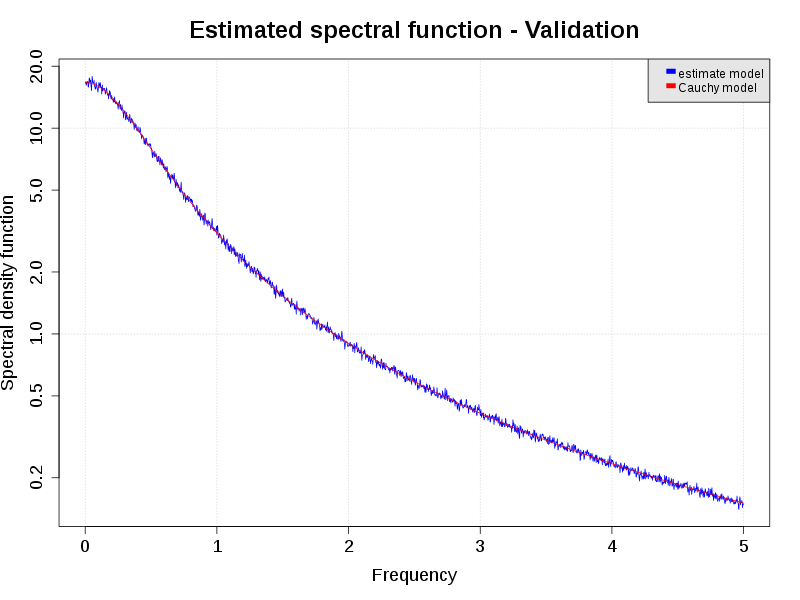
\includegraphics[width=7cm]{Figures/welchValidation.png}
    \caption{Comparison of spectral density : estimation with the Welch method vs Cauchy Model}
    \label{welch_validation}
  \end{center}
\end{figure}
